\documentclass[leqno,11pt]{article}
\usepackage{a4wide}
\usepackage[T1]{fontenc}
\usepackage[utf8]{inputenc}
\usepackage{graphicx}
\usepackage{amssymb}
\usepackage{url}
%\textwidth 19cm
%\oddsidemargin -1.54cm

\setlength\parskip{0.13in}

\title{ocd - ocd c decompiler}
\date{\today}

\begin{document}
\maketitle

\tableofcontents

\newpage

\section{Introduction}

ocd is a C decompiler written in Python, currently supporting decompilation of programs compiled for the x64 architecture. The internal data structures used for instructions are quite universal, so it should be trivial to add additional architectures as they are needed, as well as new output languages. The decompiler performs some inferences as to the program structure (such as control and data flow analysis).

\section{Using ocd}

ocd reads a specified object file, performs decompilation on it and prints the results on standard output. It can also output a set of control flow graphs in dot format. 
\\ The usage of the program is as follows:

\begin{verbatim}
Usage: ocd.py [options] file

Options:
  -h, --help            show this help message and exit
  -d OPTION, --debug=OPTION
                        turn debug option on
  -g FILE, --graph=FILE
                        output a control flow graph
\end{verbatim}


An example control flow graph looks like this:

\includegraphics[width=15cm]{images/cfg_example.eps}

\section{Operation}

\subsection{Overview}

The decompilation occurs in stages. The program is built to be modular and each stage is separate. The stages are shown in figure \ref{fig:graph_stages}.

\begin{figure}
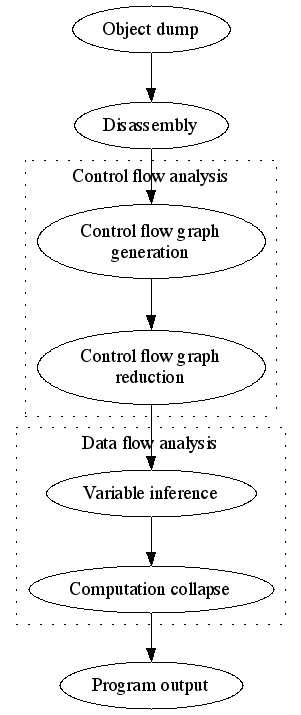
\includegraphics[height=10cm]{images/graph_stages.eps}
\centering
\caption{Stages of decompilation}
\label{fig:graph_stages}
\end{figure}

\subsection{Control flow analysis}

\section{Contributing to ocd}

ocd uses git as its SCM. The master repository is hosted at \url{http://github.com/drx/ocd}. If you want to contribute to the project, you can ask the current maintainer to add you to the contributors list. Alternatively, you can fork the project and then request that your changes be merged to the original project.

\section{Copyright}

\begin{verbatim}
 Copyright (c) 2010 Alek Balicki, Łukasz Zapart

 Permission is hereby granted, free of charge, to any person
 obtaining a copy of this software and associated documentation
 files (the "Software"), to deal in the Software without
 restriction, including without limitation the rights to use,
 copy, modify, merge, publish, distribute, sublicense, and/or sell
 copies of the Software, and to permit persons to whom the
 Software is furnished to do so, subject to the following
 conditions:

 The above copyright notice and this permission notice shall be
 included in all copies or substantial portions of the Software.

 THE SOFTWARE IS PROVIDED "AS IS", WITHOUT WARRANTY OF ANY KIND,
 EXPRESS OR IMPLIED, INCLUDING BUT NOT LIMITED TO THE WARRANTIES
 OF MERCHANTABILITY, FITNESS FOR A PARTICULAR PURPOSE AND
 NONINFRINGEMENT. IN NO EVENT SHALL THE AUTHORS OR COPYRIGHT
 HOLDERS BE LIABLE FOR ANY CLAIM, DAMAGES OR OTHER LIABILITY,
 WHETHER IN AN ACTION OF CONTRACT, TORT OR OTHERWISE, ARISING
 FROM, OUT OF OR IN CONNECTION WITH THE SOFTWARE OR THE USE OR
 OTHER DEALINGS IN THE SOFTWARE.
\end{verbatim}


\end{document}
